% Shared standalone design for the editable figure reconstructions.
\documentclass[tikz,border=5pt,10pt]{standalone}
\usepackage[T1]{fontenc}
\usepackage[utf8]{inputenc}
\usepackage{newpxtext,newpxmath}
\usepackage[scaled=.94]{sourcesanspro}
\usepackage{pgfplots}
\pgfplotsset{compat=1.18}
\usetikzlibrary{arrows.meta,calc,positioning,decorations.pathreplacing,
  decorations.markings,patterns,matrix,shapes.geometric,fit,backgrounds,
  intersections,angles,quotes}
\definecolor{ink}{HTML}{203746}
\definecolor{accent}{HTML}{146C78}
\definecolor{muted}{HTML}{667780}
\definecolor{signalred}{HTML}{B94B44}
\color{ink}
\tikzset{>=Latex,line width=.8pt,
  every node/.style={font=\small},
  axis/.style={->,draw=muted,line width=.5pt},
  guide/.style={draw=muted,dashed,line width=.45pt},
  curve/.style={draw=accent,line width=1pt},
  marker/.style={circle,fill=accent,inner sep=1.5pt},
  labelbox/.style={fill=white,inner sep=2pt}}

\begin{document}
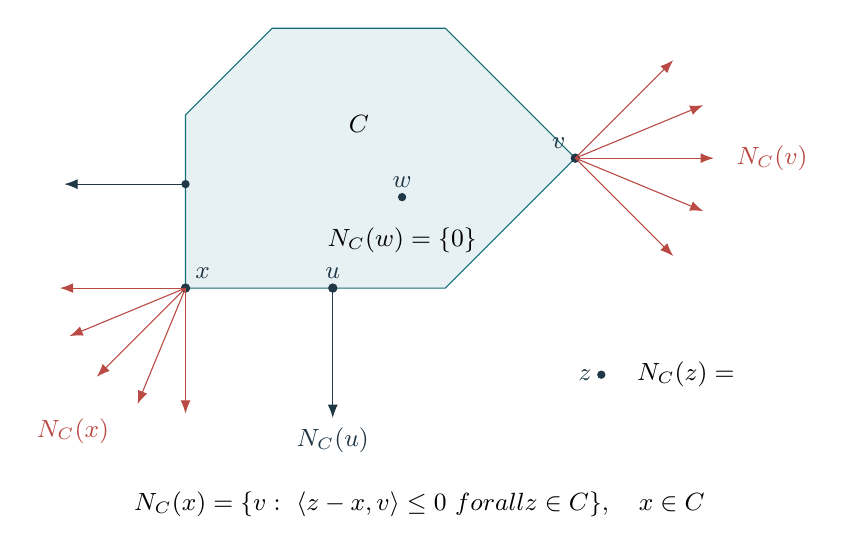
\begin{tikzpicture}[x=1.1cm,y=1.1cm]
\path[draw=accent,fill=accent!10](0,0)--(3,0)--(4.5,1.5)--(3,3)--(1,3)--(0,2)--cycle;
\node at(2,1.9){$C$};
\fill[ink](0,0)circle(1.7pt)node[above right]{$x$};
\foreach \a in {180,202.5,225,247.5,270}{\draw[->,signalred](0,0)--({1.45*cos(\a)},{1.45*sin(\a)});}
\node[signalred]at(-1.3,-1.65){$N_C(x)$};
\fill[ink](1.7,0)circle(1.7pt)node[above]{$u$};\draw[->,ink](1.7,0)--(1.7,-1.5)node[below]{$N_C(u)$};
\fill[ink](0,1.2)circle(1.5pt);\draw[->,ink](0,1.2)--(-1.4,1.2);
\fill[ink](4.5,1.5)circle(1.7pt)node[above left]{$v$};
\foreach \a in {-45,-22.5,0,22.5,45}{\draw[->,signalred](4.5,1.5)--({4.5+1.6*cos(\a)},{1.5+1.6*sin(\a)});}
\node[signalred,anchor=west]at(6.25,1.5){$N_C(v)$};
\fill[ink](2.5,1.05)circle(1.5pt)node[above]{$w$};\node at(2.5,.55){$N_C(w)=\{0\}$};
\fill[ink](4.8,-1)circle(1.5pt)node[left]{$z$};\node[right]at(5.1,-1){$N_C(z)=\varnothing$};
\node at(2.7,-2.5){$N_C(x)=\{v:\ \langle z-x,v\rangle\leq0\ \text{for all }z\in C\},\quad x\in C$};
\end{tikzpicture}
\end{document}
